% Options for packages loaded elsewhere
\PassOptionsToPackage{unicode}{hyperref}
\PassOptionsToPackage{hyphens}{url}
\PassOptionsToPackage{dvipsnames,svgnames,x11names}{xcolor}
%
\documentclass[
]{aft}

\usepackage{amsmath,amssymb}
\usepackage{iftex}
\ifPDFTeX
  \usepackage[T1]{fontenc}
  \usepackage[utf8]{inputenc}
  \usepackage{textcomp} % provide euro and other symbols
\else % if luatex or xetex
  \usepackage{unicode-math}
  \defaultfontfeatures{Scale=MatchLowercase}
  \defaultfontfeatures[\rmfamily]{Ligatures=TeX,Scale=1}
\fi
\usepackage{lmodern}
\ifPDFTeX\else  
    % xetex/luatex font selection
\fi
% Use upquote if available, for straight quotes in verbatim environments
\IfFileExists{upquote.sty}{\usepackage{upquote}}{}
\IfFileExists{microtype.sty}{% use microtype if available
  \usepackage[]{microtype}
  \UseMicrotypeSet[protrusion]{basicmath} % disable protrusion for tt fonts
}{}
\makeatletter
\@ifundefined{KOMAClassName}{% if non-KOMA class
  \IfFileExists{parskip.sty}{%
    \usepackage{parskip}
  }{% else
    \setlength{\parindent}{0pt}
    \setlength{\parskip}{6pt plus 2pt minus 1pt}}
}{% if KOMA class
  \KOMAoptions{parskip=half}}
\makeatother
\usepackage{xcolor}
\setlength{\emergencystretch}{3em} % prevent overfull lines
\setcounter{secnumdepth}{5}
% Make \paragraph and \subparagraph free-standing
\makeatletter
\ifx\paragraph\undefined\else
  \let\oldparagraph\paragraph
  \renewcommand{\paragraph}{
    \@ifstar
      \xxxParagraphStar
      \xxxParagraphNoStar
  }
  \newcommand{\xxxParagraphStar}[1]{\oldparagraph*{#1}\mbox{}}
  \newcommand{\xxxParagraphNoStar}[1]{\oldparagraph{#1}\mbox{}}
\fi
\ifx\subparagraph\undefined\else
  \let\oldsubparagraph\subparagraph
  \renewcommand{\subparagraph}{
    \@ifstar
      \xxxSubParagraphStar
      \xxxSubParagraphNoStar
  }
  \newcommand{\xxxSubParagraphStar}[1]{\oldsubparagraph*{#1}\mbox{}}
  \newcommand{\xxxSubParagraphNoStar}[1]{\oldsubparagraph{#1}\mbox{}}
\fi
\makeatother


\providecommand{\tightlist}{%
  \setlength{\itemsep}{0pt}\setlength{\parskip}{0pt}}\usepackage{longtable,booktabs,array}
\usepackage{calc} % for calculating minipage widths
% Correct order of tables after \paragraph or \subparagraph
\usepackage{etoolbox}
\makeatletter
\patchcmd\longtable{\par}{\if@noskipsec\mbox{}\fi\par}{}{}
\makeatother
% Allow footnotes in longtable head/foot
\IfFileExists{footnotehyper.sty}{\usepackage{footnotehyper}}{\usepackage{footnote}}
\makesavenoteenv{longtable}
\usepackage{graphicx}
\makeatletter
\def\maxwidth{\ifdim\Gin@nat@width>\linewidth\linewidth\else\Gin@nat@width\fi}
\def\maxheight{\ifdim\Gin@nat@height>\textheight\textheight\else\Gin@nat@height\fi}
\makeatother
% Scale images if necessary, so that they will not overflow the page
% margins by default, and it is still possible to overwrite the defaults
% using explicit options in \includegraphics[width, height, ...]{}
\setkeys{Gin}{width=\maxwidth,height=\maxheight,keepaspectratio}
% Set default figure placement to htbp
\makeatletter
\def\fps@figure{htbp}
\makeatother

\usepackage{booktabs}
\usepackage{longtable}
\usepackage{array}
\usepackage{multirow}
\usepackage{wrapfig}
\usepackage{float}
\usepackage{colortbl}
\usepackage{pdflscape}
\usepackage{tabu}
\usepackage{threeparttable}
\usepackage{threeparttablex}
\usepackage[normalem]{ulem}
\usepackage{makecell}
\usepackage{xcolor}
\usepackage{orcidlink}
\definecolor{mypink}{RGB}{219, 48, 122}
\makeatletter
\@ifpackageloaded{caption}{}{\usepackage{caption}}
\AtBeginDocument{%
\ifdefined\contentsname
  \renewcommand*\contentsname{Table of contents}
\else
  \newcommand\contentsname{Table of contents}
\fi
\ifdefined\listfigurename
  \renewcommand*\listfigurename{List of Figures}
\else
  \newcommand\listfigurename{List of Figures}
\fi
\ifdefined\listtablename
  \renewcommand*\listtablename{List of Tables}
\else
  \newcommand\listtablename{List of Tables}
\fi
\ifdefined\figurename
  \renewcommand*\figurename{Figure}
\else
  \newcommand\figurename{Figure}
\fi
\ifdefined\tablename
  \renewcommand*\tablename{Table}
\else
  \newcommand\tablename{Table}
\fi
}
\@ifpackageloaded{float}{}{\usepackage{float}}
\floatstyle{ruled}
\@ifundefined{c@chapter}{\newfloat{codelisting}{h}{lop}}{\newfloat{codelisting}{h}{lop}[chapter]}
\floatname{codelisting}{Listing}
\newcommand*\listoflistings{\listof{codelisting}{List of Listings}}
\makeatother
\makeatletter
\makeatother
\makeatletter
\@ifpackageloaded{caption}{}{\usepackage{caption}}
\@ifpackageloaded{subcaption}{}{\usepackage{subcaption}}
\makeatother

\ifLuaTeX
  \usepackage{selnolig}  % disable illegal ligatures
\fi
\usepackage[]{natbib}
\bibliographystyle{te}
\usepackage{bookmark}

\IfFileExists{xurl.sty}{\usepackage{xurl}}{} % add URL line breaks if available
\urlstyle{same} % disable monospaced font for URLs
\hypersetup{
  pdftitle={Modeling Longitudinal Binary Outcomes in a Small Matched-Pair Sample with Application to Cardiovascular Data: A Simulation Study},
  pdfauthor={Jinyu Luo; Chun-Po Steve Fan; Sudipta Saha; Aya Mitani},
  pdfkeywords={GEE, QLS, longitudinal},
  colorlinks=true,
  linkcolor={blue},
  filecolor={Maroon},
  citecolor={Blue},
  urlcolor={red},
  pdfcreator={LaTeX via pandoc}}



\title{Modeling Longitudinal Binary Outcomes in a Small Matched-Pair
Sample with Application to Cardiovascular Data: A Simulation Study}
\author{
Jinyu Luo~\orcidlink{0009-0004-1101-7040}\\University of
Toronto\\\href{mailto:jinyu.luo@mail.utoronto.ca}{jinyu.luo@mail.utoronto.ca}\and 
Chun-Po Steve Fan~\orcidlink{0000-0002-6373-0532}\\University Health
Network\\\href{mailto:steve.fan@uhn.ca}{steve.fan@uhn.ca}\and 
Sudipta Saha\\University Health
Network\\\href{mailto:Sudipta.Saha@uhn.ca}{Sudipta.Saha@uhn.ca}\and 
Aya Mitani~\orcidlink{0000-0002-0373-5032}\\University of
Toronto\\\href{mailto:aya.mitani@utoronto.ca}{aya.mitani@utoronto.ca}}
\date{}
\begin{document}
\maketitle
\begin{abstract}
This study aimed to address the challenge of modeling small sample
matched-pair longitudinal data in cardiovascular research. The
independent working correlation structure in Generalized Estimating
Equations (GEE), a robust method widely used for modeling endogenous
follow-up data, relies on large-sample theory. Prior research has noted
significant constraints due to small sample sizes for continuous
outcomes. We evaluated the performance and validity of the GEE method
and the two-stage quasi-least squares (QLS) approach in analyzing small
matched-pair longitudinal binary data, particularly focusing on the
interaction effect between bicuspid aortic valve (BAV) and time on
aortic root size post-surgery. Hospital cohorts with longitudinal
outcomes across two exposure groups were matched using propensity scores
based on baseline characteristics to eliminate potential confounding
effects, which is followed by GEE fit assuming that working correlation
structure is AR1 to get a set of regression coefficients for simulation
parameters. Simulations were designed to mimic real-world dropout
processes, where previous survival outcomes and associated covariates
influence longitudinal outcomes. Standard errors were adjusted by
degrees of freedom to prevent underestimation by the sandwich estimator.
Results: The QLS method demonstrated superior performance, with mean
estimates closer to the true coefficients and narrower confidence
intervals than GEE, while GEE provided more accurate estimation for the
interaction effect but exhibited higher variability in estimates. Both
methods struggled to capture the effect of time. Including confounding
covariates did not significantly impact performance. QLS provided more
consistent estimates across different correlation structures but with
higher bias. Conclusion: Proper specification of the correlation
structure is crucial for the robust analysis of small sample
longitudinal data. For studies with small sample sizes and complex
correlation structures, QLS may offer a more reliable alternative by
providing consistent estimates with lower variability. These findings
underscore the importance of methodological considerations in
longitudinal data analysis and offer guidance for selecting appropriate
analytical approaches.
\end{abstract}


\section{Introduction}\label{sec-intro}

The generalized estimating equations (GEE) method is commonly used in
longitudinal studies where the response variable for each subject is
measured repeatedly over time \citep{LiangZeger1986}. It is an extension
of the quasi-likelihood method that models the marginal expectation of
the response, either discrete or binary, as a function of a set of
explanatory variables \citep{Agresti2nd}. Instead of assuming a
particular type of distribution for the outcome \(Y\), each marginal
mean is linked to a linear predictor and educated guess for the
variance-covariance structure, which accounts for the temporal
correlation among repeated measurements. Since there is no need to
specify the random effects for individual subjects or clusters, GEE
provides an average response in the population rather than
individual-specific effects.

Our motivation stems from the work which assessed the natural history of
the aortic root in patients with bicuspid versus tricuspid aortic valves
(BAVs vs.~TAVs) after replacement of the aortic valve and ascending
aorta at the Peter Munk Cardiac Center \citep{Hui2018}. The aorta is the
main artery that carries blood from the heart's left ventricle to the
rest of the human body. According to the 2014 ESC guidelines on
diagnosing and treating aortic diseases, aorta dilatation is a clinical
condition with aorta diameter greater than 40 mm, irrespective of body
surface area. It is commonly present in patients with BAV, a congenital
heart defect when the aortic valve has only two leaflets instead of
three and affects approximately 1-2\% of the general population
\citep{Wang2021}. Patients with aortic diameter exceeding 4.5 mm are
usually associated with ascending aortic events. Evidence showed that
the dilation of aortic root cannot be suppressed even after AVR
\citep{Bruce2003}. Still, other researchers found that the ascending
aorta dilatation rate was similar between the BAV and TAV post-surgery
\citep{KIM202053}.

Given that BAV is a congenital cardiac abnormality, conducting
randomized controlled trials is not feasible. Researchers often pair BAV
patients with TAV patients using propensity score matching (PSM) to
assess the natural history of aortic root size changes. PSM is critical
in this context as it balances observed covariates between BAV and TAV
groups, reducing confounding bias and enhancing the accuracy of
treatment effect estimates. This technique allows for valid comparisons
in observational studies, addressing selection bias and leading to more
reliable conclusions about the natural history of aortic root size
changes post-surgery. In practice, patients with and without exposure to
interest are matched on important confounding factors such as age, sex,
and calendar time and compared for the incidence of outcomes
\citep{Iwagami2022}. In such a scenario, two distinct correlations
exist: the correlation between units within the matched pair and the
correlation between the temporal observations on the same patient.

The study investigators collected participant-level demographics, health
outcomes, and each participant's follow-up imaging data after the
replacement of the aortic valve (AVR) and ascending aorta (RAA) from
January 1900 to December 2010. This cohort consists of 406 patients, 244
of whom had follow-up measurements. Among those with follow-up visits,
172 (70.5\%) patients had BAV, and the rest had TAV. Our primary outcome
is whether or not the aortic root dimensions exceeded a diameter of 45
mm after the surgery. Although the data include records of patients'
vitals, only the follow-up measurements of the aortic root size and
baseline covariates, including age, sex, and body surface area (BSA),
are included in this study.

The first consideration in GEE analysis is the potential issue of
covariate endogeneity. This concept describes the scenario when the
response at time \(t\) predicts the covariate value at times \(s > t\)
\citep{Diggle2002}. The issue arises because the abnormal aortic root
size is associated with a higher risk of death \citep{KITAGAWA2013258},
and the occurrence of death informs that there is no stochastic process
of the deformation. The interaction effect between response and
covariates is called \emph{feedback} \citep{Zeger1991}. It has been
shown that, based on the large-sample theory, using GEE with a working
independence correlation structure can provide unbiased estimation
\citep[@LiangZeger1986]{Diggle2002}. However, the sample sizes in
cardiovascular research are limited and mid-term follow-ups are
incomplete due to the rarity of disease in practice. The validity of GEE
with a working independence correlation structure remains unknown. The
second consideration is that GEE methods within the existing R package,
i.e., \texttt{geepack,} only account for the correlation between
repeated measurements within one subject but ignore the correlation
between matched pairs.

This report focuses on matched longitudinal binary data with covariate
endogeneity and informative dropouts. We aim to explore the validity of
GEE estimates for small sample matched-pair binary outcomes and compare
the estimation results with the two-stage quasi-least squares (QLS)
method \citep{Mitani2019}. In section 2, notations and assumptions are
first presented, followed by a description of the issue with the
correlation structure within the GEE framework, the construction of the
two-stage QLS method, and the pre-processing of the motivational data.
The simulation study design is presented in section 3. Section 4
presents an analysis of the motivational data and simulation results.
Finally, we conclude this report with a discussion in section 5.

\section{Methods}\label{methods}

\subsection{Notation and Assumptions}\label{notation-and-assumptions}

Consider a longitudinal matched data set in which subjects are grouped
into pairs, and each subject contributes repeated observations of unique
aortic root diameter. Let
\(\boldsymbol{Y}'_{ij} = (Y_{ij1}, Y_{ij2}, ..., Y_{ijt_{ij}})\) be a
vector of measurements for subject \(j\) in matched pair \(i\) at times
\(t_{ij1}, t_{ij2}, ..., t_{ijT}\), where
\(t_{ij1} < t_{ij2} < \cdots < t_{ijT}\); \(i = 1,..., m\);
\(j = 1, 2\); \(k = 1,...,T\). Associated with each \(Y_{ijk}\) is a
vector of covariates
\(\boldsymbol{X}'_{ijk} = (X_{ijk1}, X_{ijk2}, X_{ijk3})\) corresponding
to BAV (exposure), \emph{time}, and the interaction between BAV and
\emph{time}. Note that BAV is the exposure variable which is diagnosed
before this study and does not change by time. Additionally, since
different patients may have different follow-up intervals, we define
\emph{time} as the number of visits. The outcome \(Y_{ijk}\) have mean
and variance \[
E(Y_{ijk} | X_{ijk}) = \mu_{ijk} \quad \text{and} \quad Var(Y_{ijk}) = \mu_{ijk}(1-\mu_{ijk}) = h(\mu_{ijk})
\]

Our analysis goal is to examine the effect of these covariates on the
marginal mean of the binary outcome through
\(g^{-1}(\boldsymbol{X}_{ijk}'\boldsymbol{\beta})\), where
\(\boldsymbol{\beta} = (\beta_0, \beta_1, \beta_2,\beta_3)\) are unknown
regression coefficients and \(g(\cdot)\) is the invertible link function
which is defined as \[
\begin{aligned}
g(\mu_{ijk}) &= \log(\frac{\mu_{ijk}}{1-\mu_{ijk}}) \\
&= \beta_0 + \beta_1\cdot \text{BAV}_{ijk} + \beta_2 \cdot \text{Time}_{ijk} + \beta_3\cdot (\text{BAV}_{ijk} \times \text{Time}_{ijk})\\
&= X_{ij}'\boldsymbol{\beta}.
\end{aligned}
\]

We assume that observations from different matched pairs are independent
but are correlated within the same pair. The variance matrix of
\(\boldsymbol{Y}_i' = (Y_{i1}'. Y_{i2}')\) is given by \[
\Sigma_i = A_i^{1/2}(\beta) F_i(\Gamma) A_i^{1/2} (\beta) 
\] where \(F_i(\Gamma)\) is the positive definite working correlation
matrix of the vector of outcome for pair \(i\), \(\Gamma\) is a vector
of unknown correlation parameters, and \begin{align}
A_i(\beta) &= \text{diag}\left\{A_{i1}(\beta), A_{i2}(\beta)\right\} \label{eq: Aibeta}\\
A_{ij}(\beta) & = \text{diag}\left\{h(\mu_{ij1}), h(\mu_{ij2}),...,h(\mu_{ijT})\right\} \label{eq: Aij}.
\end{align}

\subsection{Generalized estimating equations
(GEE)}\label{generalized-estimating-equations-gee}

Without a specific assumption about the likelihood function, generalized
estimating equations (GEE) accounts the covariance structure of the
repeated measures by specifying a working correlation matrix,
\(R(\alpha)\), which describes the correlation between repeated measures
on the same subject. This paper focuses on the following three working
correlations: \[
\underset{\text{(Independent)}}{\begin{bmatrix}
1 & 0 & \cdots & 0\\
0 & 1 & \cdots &  0\\
\vdots & \vdots & \ddots & \vdots\\
0 & 0 & \cdots & 1
\end{bmatrix}}
\quad
\underset{\text{(Exchangeable)}}{\begin{bmatrix}
1 & \alpha & \cdots & \alpha\\
\alpha & 1 & \cdots & \alpha\\
\vdots & \vdots & \ddots & \vdots\\
\alpha & \alpha & \cdots & 1
\end{bmatrix}}
\quad
\underset{\text{(AR1)}}{\begin{bmatrix}
1 & \alpha & \cdots & \alpha^{t_{ij} - 1}\\
\alpha & 1 & \cdots & \alpha^{t_{ij} - 2}\\
\vdots & \vdots & \ddots & \vdots\\
\alpha^{t_{ij} - 1} & \alpha^{t_{ij} - 2} & \cdots & 1
\end{bmatrix}}
\] . The independent working correlation assumes no correlation between
repeated measures. With a correlation coefficient \(\alpha\), the
exchangeable working correlation assumes that the correlation between
any pair of repeated measurements are constant at \(\alpha\), whereas
the autoregressive order one (AR1) working correlation structure assumes
correlation decreases exponentially with the time lag between measures.

GEE approach accounts for overdispersion or underdispersion by
correcting the variance using a dispersion parameter \[
\text{Var}(Y_{ijk})^* = \phi\text{Var}(Y_{ijk}) = \phi h(\mu_{ijk})
\] Since our outcome is binary, the dispersion parameter \(\phi\) equals
to 1.

The iterative process starts with initial guesses for the regression
coefficients \(\boldsymbol{\beta}^{(0)}\) and the correlation parameters
\(\alpha^{(0)}\). It is followed by the computation of initial marginal
expectation
\(\mu_{ijk}^{(0)} = g^{-1}(X_{ijk}^T \boldsymbol{\beta}^{(0)})\), where
\(g^{-1}\) is the inverse of the link function. Then, the iterative
process mainly consists of two steps: (1) update the working correlation
matrix using the sample data. (2) update the regression coefficients.

\subsubsection{Update the Working Correlation
Matrix}\label{update-the-working-correlation-matrix}

To update the working correlation matrix, we first compute the
residuals, \(r_{ijk}^{(m)} = Y_{ijk} - \mu_{ijk}^{(m)}\), based on the
current estimates of the marginal means for each observation. Then, we
estimate the correlation parameters using the residuals and construct
the working correlation matrix \(R_i^{(m)}(\alpha^{(m)})\) using the
updated correlation parameters.

\subsubsection{Update the Regression
Coefficients}\label{update-the-regression-coefficients}

The problem with GEE approach is that it does not account for the
correlation between subjects within the same matched pair, so the
variance matrix is simplified to \begin{equation}
\Sigma_i(\alpha) = A_i^{1/2}(\beta)R(\alpha)A_i^{1/2}(\beta) \label{eq:geeCovMat}
\end{equation} where \(A_i^{1/2}\) is defined in \eqref{eq: Aibeta}.
Then, the score function and the information matrix can be calculated
using the current estimates \citep{Zeger1988}: \begin{align}
\boldsymbol{S}(\boldsymbol{\beta}) &= \sum_{i=1}^m D_i^T \Sigma_i^{-1}(\alpha) (Y_i - \mu_i) \label{eq:geeScoreEqs}\\
I(\boldsymbol{\beta}) &= \sum_{i=1}^m D_i^T\Sigma_i^{-1}(\alpha)D_i \label{eq:geeInfoMat}
\end{align} where \begin{equation}
D_i = \frac{\partial \boldsymbol{U}_i}{\partial \boldsymbol{\beta}} = \frac{\exp(\boldsymbol{X}_i\boldsymbol{\beta})}{1+\exp(\boldsymbol{X}_i \boldsymbol{\beta})}. \label{eq:Di}
\end{equation} The new set of regression coefficients are obtained by
solving the score function, which are then used to calculate the new
marginal means.

The final estimates of the regression coefficients
\(\boldsymbol{\beta}\) can be obtained by repeat the above process until
convergence is achieved \citep{Liang1986}. This iterative process
ensures that the correlation structure and the regression coefficients
are appropriately updated using the sample data, resulting in consistent
and efficient parameter estimates in the presence of correlated repeated
measures.

However, it has been shown that the sandwich estimator tends to
underestimate standard errors (SEs) when the size sample data is small
\citep{Mitani2019}. To overcome this issue, we can adjust the sandwich
estimator by degrees of freedom \citep{dfcorrect}: \begin{equation}
\Sigma_{DF} = (\frac{2m}{2m-p})\Sigma \label{eq:geeSigmaDF}
\end{equation} where \(2m\) represents the number of patients, \(p\) is
the number of regression parameters.

\subsection{Quasi-least squares (QLS)}\label{quasi-least-squares-qls}

Quasi-least squares (QLS) is a two-stage approach for estimating the
correlation parameters in the framework of generalized estimating
equations (GEE). The method involves estimating the regression
parameters and the correlation structure in two distinct stages.
Proposed by \citet{qls}, the two-stage QLS method assumes that the
covariance matrix are functions of the regression parameters and
independent of the dispersion parameter \(\phi\). Additionally, the
off-diagonal elements are functions of some unknown nuisance parameters.
The first stage mainly aims to estimate the regression parameters by
minimizing the score function, which is consistent with the GEE
approach. The difference is that the QLS method solves an unbiased
estimating equation for \(\alpha\), whereas the GEE method implements
moment estimates of the correlation parameters \citep{qlspack}. The
second stage refines the estimates of the correlation parameters based
on the residuals from the first stage and updates the working
correlation matrix. By iterating between these two stages, the two-stage
QLS approach ensures robust and efficient estimates of the regression
parameters while appropriately accounting for the correlation within the
data.

This study adopted the method proposed by \citet{Shults2002} which
specified the working correlation structure by incorporating both
intravisit and intrapair correlations using equicorrelated matrices and
the Kronecker product. Let the working correlation parameter
\(\Gamma' = (\boldsymbol{\tau}', \boldsymbol{\alpha}')\) where
\(\boldsymbol{\tau}' = (\tau_1, ..., \tau_m)\) account for the
correlation between subjects for each matched pairs and
\(\boldsymbol{\alpha}' = (\alpha_1, \alpha_2)\) is the vector of
correlation coefficients for longitudinal measurements within the a
subject in a pair. In this study, we assume that the intra-pair
correlations are consistent across different pairs, that is,
\(\tau_1 = \tau_2 = ... = \tau_m = \tau\). Let
\(R_i(\boldsymbol{\alpha}) = \{r^i_{jk}(\boldsymbol{\alpha})\}\) be a
\(T \times T\) intravisit working correlation matrix for outcomes
collected on subjects \(j\) from pair \(i\) and \(Q_i(\tau)\) be a
\(2 \times 2\) equicorrelated working correlation matrix with all
off-diagonal elements equal to \(\tau_i\). We assume that
\(F_i(\Gamma)\) is the Kronecker product of \(Q_i(\tau)\) and
\(R_i(\boldsymbol{\alpha})\), denoting as
\(Q_i(\tau)\otimes R_i(\boldsymbol{\alpha})\).

Let \(z_{ijk}\) be the standardized residual for the \(k\)-th visit on
the \(j\)-th subject from the \(i\)-th pair, written as \[
z_{ijk} = \frac{Y_{ijk} - \mu_{ijk}}{\sqrt{h(\mu_{ijk})}}.
\] Let \(Z_{ij}'\) be a vector of standardized residuals and \(U_{ij}'\)
be a vector of mean values of longitudinal outcomes for the \(j\)-th
subject form the \(i\)-th pair, then
\(Z_i'(\beta) = (Z_{i1}', Z_{i2}')\) is a vector of all standardized
residuals and \(\boldsymbol{U}_i' = (U_{i1}', U_{i2}')\) is a vector of
all expected outcomes within \(i\)-th pair. Now, the generalized error
sum of squares is expressed as \[
Q(\boldsymbol{\beta}, \boldsymbol{\Gamma}) = \sum_{i=1}^m Z_i'(\beta)F_i^{-1}(\Gamma) Z_i(\beta)
\]

\subsubsection{\texorpdfstring{Estimation of
\(\beta\)}{Estimation of \textbackslash beta}}\label{estimation-of-beta}

The estimating equation for \(\boldsymbol{\beta}\) can be obtained by
taking the partial derivative of
\(Q(\boldsymbol{\beta}, \boldsymbol{\Gamma})\) with respect to
\(\boldsymbol{\beta}\) and setting it equal to 0: \[
\begin{aligned}
\frac{\partial Q(\boldsymbol{\beta}, \boldsymbol{\Gamma})}{\partial \boldsymbol{\beta}} &= 2 \sum_{i=1}^m \boldsymbol{D}_i'(\boldsymbol{\beta})F_i^{-1}(\boldsymbol{\Gamma})\boldsymbol{Z}_i(\boldsymbol{\beta})\\
&= 2\sum_{i=1}^m \boldsymbol{D}_i'(\boldsymbol{\beta})F_i^{-1}(\boldsymbol{\Gamma})\left(\frac{\boldsymbol{Y}_i - \boldsymbol{U}_i}{\sqrt{h(\boldsymbol{U}_i)}}\right)
\end{aligned}
\] Then, we have \begin{equation}
\sum_{i=1}^m \boldsymbol{D}_i'(\boldsymbol{\beta})F_i^{-1}(\boldsymbol{\Gamma})\left(\frac{\boldsymbol{Y}_i - \boldsymbol{U}_i}{\sqrt{h(\boldsymbol{U}_i)}}\right) = 0, \label{eq:qlsdQdb}
\end{equation} where \(\boldsymbol{D}_i\) is defined in \eqref{eq:Di}.

\subsubsection{\texorpdfstring{Estimation of
\(\Gamma\)}{Estimation of \textbackslash Gamma}}\label{estimation-of-gamma}

The partial derivative of \(Q(\boldsymbol{\beta}, \boldsymbol{\Gamma})\)
with respect to \(\boldsymbol{\Gamma}\) can be divided into two parts:
taking partial derivative with respect to \(\tau\) and \(\alpha\)
separately. Since the stage one estimation is is asymptotically biased
\citep{CHAGANTY1999145}, the estimation for \(\tau\) and \(\alpha\)
involves two stages for each.

\textbf{Stage One Estimators}

As defined earlier, \[
Q_i(\tau) = 
\begin{bmatrix}
1 & \tau\\
\tau & 1
\end{bmatrix}
\implies 
Q_i^{-1}(\tau) = \frac{1}{1-\tau^2}
\begin{bmatrix}
1 & -\tau\\
-\tau & 1
\end{bmatrix}
\] Let \(q_1 = \frac{1}{1-\tau^2}\) and
\(q_2 = \frac{-\tau}{1-\tau^2}\), then we can obtain the first stage
estimator for \(\tau\) by \begin{align}
\frac{\partial}{\partial \tau}& \left\{
\sum_{i=1}^m 
\begin{pmatrix}
Z_{i1} & Z_{i2}
\end{pmatrix} 
\left[\begin{pmatrix}
q_1 & q_2\\
q_2 & q_1
\end{pmatrix} 
\otimes R_i^{-1}(\alpha)\right] 
\begin{pmatrix}
Z_{i1}\\ Z_{i2}
\end{pmatrix} \right\} = 0 \\
\sum_{i=1}^m &  \frac{\partial}{\partial \tau}\left[q_1(Z_{i1}R_i^{-1}Z_{i1}+Z_{i2}R_i^{-1}Z_{i2}) + 2q_2(Z_{i1}R_i^{-1}Z_{i2})\right]= 0 \label{eq:tau1}
\end{align} Let \(a_1 = (Z_{i1}R_i^{-1}Z_{i1}+Z_{i2}R_i^{-1}Z_{i2})\)
and \(a2 = (Z_{i1}R_i^{-1}Z_{i2})\), the stage one estimator for
\(\tau\) can be obtained by solving the equation \eqref{eq:tau1}: \[
\hat{\tau}_0 = \frac{a_1 - \sqrt{a_1^2 - 4a_2^2}}{2a_2}
\]

Given that all the subjects from the motivational study underwent the
aortic root replacement surgery, it is reasonable to believe that the
correlation of longitudinal measurements is decreasing as time passes.
Therefore, AR1 is assumed to be the true working correlation structure.
Then, a closed-form solution for stage one \(\alpha\) is:
\begin{equation}
\hat{\alpha}_0 = \frac{F_a + \sqrt{(F_1+F_b)(F_a-F_b)}}{F_b} \label{eq:ar1alpha1}
\end{equation} where \[
F_a = \sum_{i=1}^N \frac{1}{2} \sum_{j=1}^2 \frac{1}{t_{ij}}\left[\sum_{k=1}^{t_{ij}} Z_{ijk}^T C_i^{-1} Z_{ijk} + \sum_{k=2}^{t_{ij}-1}Z_{ijk}^T C_i^{-1} Z_{ijk}\right]
\] and
\(F_b = 2\sum_{i=1}^N \frac{1}{2}\sum_{j=1}^2\frac{1}{t_{ij}}\sum_{k=1}^{t_{ij}-1} Z_{ijk}^T C_i^{-1} Z_{ijk+1}\).
The closed form solution for the stage two estimator of \(\alpha\) is
given by \citep{Mitani2019}: \begin{equation}
\hat{\alpha} = \frac{2\hat{\alpha}_0}{1+\hat{\alpha}_0^2} \label{eq:ar1alpha2}
\end{equation}. Details of the derivations for equation
\eqref{eq:ar1alpha1}is shown in the Appendix A.

\subsection{Modeling Motivational
Data}\label{modeling-motivational-data}

To model the motivational data, we first selected all patients who had
at least one follow-up visit with baseline measurement being taken at
the day of operation. Then, a binary outcome was created by setting it
to 1 if the current root size measurement is over 45 mm or the growth
from the previous measure is over 5 mm, and 0 otherwise. A maximal of 6
records (including the baseline) for each patient were kept for further
analysis. Then, assuming that dropouts follows Weibull distribution, 5
survival models were fitted from visit 2 to 6. The fitting coefficients
were extracted for simulation. Next, a logistic regression model is
fitted on the data which included the baseline measurements so that we
can pair BAV patients with TAV patients using the \texttt{pairmatch}
function from the R package \texttt{optmatch} \citep{optmatch}. Then, we
applied the function \texttt{geeglm} from the R package \texttt{geepack}
on the matched data set to produce the estimation results using
independence, exchangeable, and AR1 working correlation structures.
Finally, customized functions for implementing QLS are applied on the
matched data.

\section{Simulation Study}\label{simulation-study}

\subsection{Full Data Simulation}\label{full-data-simulation}

The simulation process for generating one set of cohort data involves
several steps to model both covariates and binary outcomes for each
patient. For each patient, we first simulated baseline covariates,
including age, sex, and body surface area (BSA), by assuming a normal
distribution for continuous data and a binomial distribution for binary
data. To calculate the probability of having BAV, we used a logistic
regression model of the form: \[
\text{Pr}(\text{BAV} = 1 | \text{Age, Sex, BSA}) = \frac{\exp(\gamma_0 + \gamma_1 \cdot \text{Age} + \gamma_2 \cdot \text{Sex} + \gamma_3 \text{BSA})}{1+\exp(\gamma_0 + \gamma_1 \cdot \text{Age} + \gamma_2 \cdot \text{Sex} + \gamma_3 \text{BSA})}
\] where \(\gamma_0 = -0.407, \gamma_1 = -0.071, \gamma_2 = 1.231\), and
\(\gamma_3 = 3.038\). This probability is then used to generate the
exposure variable, BAV, under binomial distribution. To simulate
longitudinal matched data with binary outcomes, the marginal probability
of having positive outcome is obtained by using another logistic
regression model that includes BAV, visit times, and their interaction:
\[
\text{Pr}(Y = 1 | \text{BAV, Visit, BAV} \times \text{Visit}) = \frac{\exp(\beta_0 + \beta_1 \cdot \text{BAV} + \beta_2 \cdot \text{Visit} + \beta_3 \cdot \text{BAV}\cdot \text{Visit})}{1+\exp(\beta_0 + \beta_1 \cdot \text{BAV} + \beta_2 \cdot \text{Visit} + \beta_3 \cdot \text{BAV}\cdot \text{Visit})}.
\] where \(\beta_0 = -1.784, \beta_1 = -1.077, \beta_2 = -0.042\) and
\(\beta_3 = 0.192\).

Each subject is assumed to have six visits, including the baseline
measurement, so six marginal probabilities are produced through this
process. The true correlation among longitudinal measurements is set to
be 0.3, and the working covariance is assumed to follow a first-order
autoregressive structure, where correlations decrease with the distance
between observations. Finally, the binary longitudinal outcomes are
generated using these marginal probabilities with the \texttt{cBern}
function within the \texttt{CorBin} package in R. This package,
developed by \citet{cbernWei}, simulates binary outcomes by ensuring a
positive definite correlation matrix and restricting the range of
correlation coefficients using Prentice constraints
\citep{Prentice1988}.

\subsection{Informative Dropout Simulation and Propensity Score
Matching}\label{informative-dropout-simulation-and-propensity-score-matching}

To simulate the informative dropouts, we first modeled the dropout
pattern by fitting the motivational data using survival models at every
visit except the baseline and the last measurement. For each visit, the
status indicator was set to 1 if the maximum number of visits for the
subject was the current visit, indicating dropout from the study with no
further follow-up measurements. For example, the first survival model
was fitted at visit 2 since visit 1 is the baseline measurement, and
subjects with a total of 2 visits were assigned a status of 1. The event
time was defined as the total number of visits. Given that the total
number of visits was 6, four survival models were fitted to the real
data. The fitting coefficients, including scale and shape parameters,
were extracted from these models. These parameters were then used in the
\texttt{simsurv} function to simulate dropouts at each follow-up visit
for the simulated data \citep{simsurv20}. Once the dropout process is
completed, propensity scores are calculated based on the logistic
regression with the three baseline covariates, which are then been
applied with the \texttt{pairmatch} function in the \texttt{optmatch} R
package to match BAV subjects with TAV subjects. Then, we applied QLS
with independence, AR1, and exchangeable working correlation structures
to estimate the regression coefficients. We also applied GEE functions
from existing R package \texttt{geepack} with the three working
correlation structures \citep{Hojsgaard2006}.

We simulated 1,000 data sets, each containing 250 subjects with up to 6
observations per subject, using the described simulation process. For
each simulation and method, we computed the mean estimates, the mean
standard errors, mean robust standard errors (MSEs), the standard
deviations (SD), mean bias, and mean relative bias for each regression
coefficient estimate. The mean bias was obtained by calculating the
difference between the mean estimates and the respective true value,
which was then divided by the true value to obtain the mean relative
bias. The coverage probability was determined by calculating the
proportion of the 95\% confidence intervals that included the respective
true parameter values among the 1,000 fitting results.

\section{Results}\label{results}

\subsection{Analysis of Motivational
Data}\label{analysis-of-motivational-data}

Table 1 compares the estimates, standard errors (SE), and SE adjusted
for degrees of freedom (SE-DF) for the GEE and QLS methods across
different working correlation structures in modeling the binary outcome
of aortic root diameter in BAV patients using data from the Peter Munk
Cardiac Center. Within each method, parameter estimates are stable
across correlation structures, showing minor variations. The GEE method
estimates for \(\beta_1\) (BAV) range from -1.093 to -1.117, while QLS
estimates range from -0.080 to -0.091. For \(\beta_2\) (Visit), GEE
estimates range from -0.052 to -0.063, and QLS estimates range from
0.007 to 0.012. The interaction term \(\beta_4\) shows a positive effect
across both methods, with GEE estimates ranging from 0.192 to 0.224 and
QLS estimates ranging from 0.009 to 0.016. The correlation parameter
\(\alpha\) are all around 1 regardless of methods and correlation
structures. Notably, the estimation for \(\tau\) is around zero in QLS,
indicating minimal within-pair correlation.

Across methods, there are notable differences in parameter estimates
within the same correlation structure. GEE consistently shows stronger
associations for BAV status and its interaction with time compared to
QLS, which yields more conservative estimates. The GEE method suggests a
stronger negative association between BAV status and the binary outcome
and a positive interaction effect between visit and BAV status, while
the QLS method indicates smaller effects.

\begin{table}[!h]
\centering\centering
\caption{\footnotesize Comparison of Estimations from GEE and QLS using longitudinal data from the Peter Munk Cardiac Center.}
\centering
\resizebox{\ifdim\width>\linewidth\linewidth\else\width\fi}{!}{
\fontsize{6}{8}\selectfont
\begin{tabular}[t]{>{}llrrrrrrrrr}
\toprule
\multicolumn{1}{c}{ } & \multicolumn{1}{c}{ } & \multicolumn{3}{c}{Independence} & \multicolumn{3}{c}{AR1} & \multicolumn{3}{c}{Exchangeable} \\
\cmidrule(l{3pt}r{3pt}){3-5} \cmidrule(l{3pt}r{3pt}){6-8} \cmidrule(l{3pt}r{3pt}){9-11}
Method & Parameter & Estimate & SE & SE-DF & Estimate & SE & SE-DF & Estimate & SE & SE-DF\\
\midrule
 & $\beta_0$ (Intercept) & -1.737 & 0.632 & 0.663 & -1.784 & 0.631 & 0.662 & -1.750 & 0.619 & 0.649\\
\cmidrule{2-11}
 & $\beta_1$ (BAV) & -1.093 & 0.811 & 0.850 & -1.077 & 0.811 & 0.851 & -1.117 & 0.787 & 0.825\\
\cmidrule{2-11}
 & $\beta_2$ (Visit) & -0.052 & 0.155 & 0.163 & -0.042 & 0.154 & 0.162 & -0.063 & 0.171 & 0.179\\
\cmidrule{2-11}
 & $\beta_4$ (Visit $\times$ BAV) & 0.195 & 0.183 & 0.192 & 0.192 & 0.182 & 0.191 & 0.224 & 0.191 & 0.200\\
\cmidrule{2-11}
\multirow[t]{-5}{*}{\raggedright\arraybackslash \textbf{GEE}} & $\alpha$ &  &  &  & 0.093 & 0.111 &  & 0.081 & 0.063 & \\
\cmidrule{1-11}
 & $\beta_0$ (Intercept) & 0.115 & 0.536 & 0.563 & 0.096 & 0.503 & 0.527 & 0.130 & 0.482 & 0.505\\
\cmidrule{2-11}
 & $\beta_1$ (BAV) & -0.084 & 0.469 & 0.492 & -0.071 & 0.482 & 0.505 & -0.108 & 0.401 & 0.420\\
\cmidrule{2-11}
 & $\beta_2$ (Visit) & 0.011 & 0.163 & 0.171 & 0.011 & 0.124 & 0.130 & -0.005 & 0.106 & 0.111\\
\cmidrule{2-11}
 & $\beta_4$ (Visit $\times$ BAV) & 0.003 & 0.189 & 0.198 & 0.007 & 0.202 & 0.212 & 0.026 & 0.125 & 0.131\\
\cmidrule{2-11}
 & $\alpha$ &  &  &  & 0.535 &  &  & 0.556 &  & \\
\cmidrule{2-11}
\multirow[t]{-6}{*}{\raggedright\arraybackslash \textbf{QLS}} & $\tau$ & 0.494 &  &  & 0.307 &  &  & 0.354 &  & \\
\bottomrule
\end{tabular}}
\end{table}

\subsection{Simulation Results}\label{simulation-results}

All 1000 simulations converged for both GEE and QLS fits. Each
simulation was checked for extreme values. Seventy-one simulations
showed extremely large standard errors when fitted with GEE, while only
nine simulations exhibited extreme standard errors using the QLS
approach. These problematic simulations were removed from further
analysis.

Figure 1 shows the average regression coefficient estimates from 1000
simulations for the GEE (left three columns) and QLS (right three
columns) methods. The estimates are presented for three covariates: BAV,
Visit, and their interaction (BAV × Visit). Each dot represents the mean
estimate across simulations, with colours indicating different working
correlation structures: AR1 (red), Exchangeable (blue), and Independence
(green). The panel labels indicate that the 95\% confidence intervals in
the first row are based on empirical standard errors, whereas the second
row uses standard errors corrected by degrees of freedom. The black
dashed line marks the true coefficient values used in the simulations.
In general, QLS shows smaller variability in estimates compared to GEE,
and both methods fail to capture the true coefficient for the effect of
Visit regardless of the adjustment for standard errors. The mean
estimates for the effect of BAV using QLS are more accurate and have
less variability, while the mean estimates for the interaction effect
using the GEE approach are closer to the true value, although they show
greater variability. More details about accurate true parameter coverage
probabilities can be found in the Appendix B.

\begin{figure}[H]

{\centering 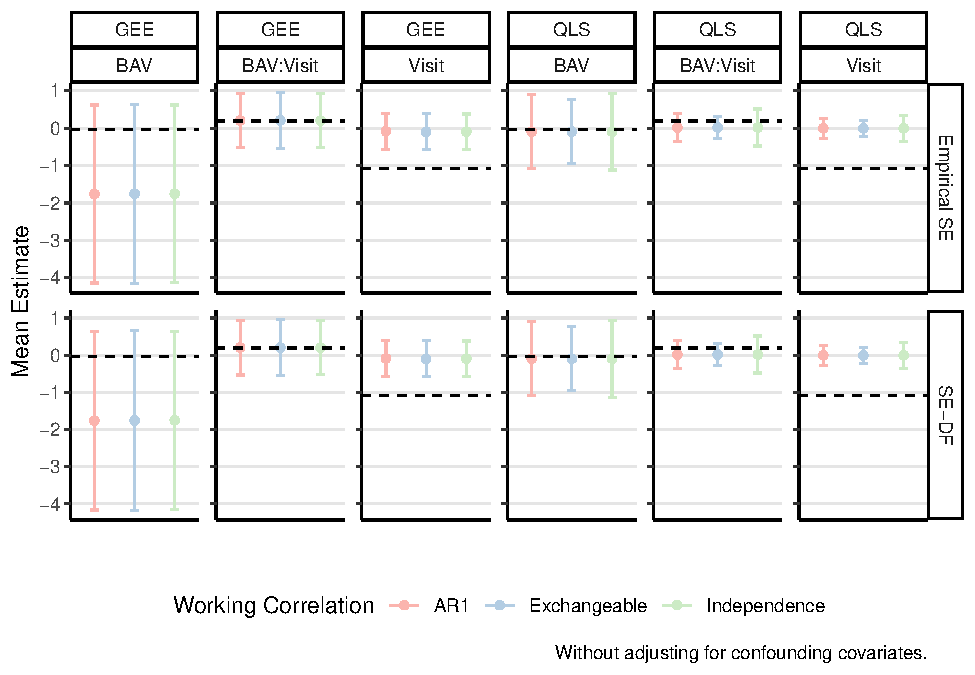
\includegraphics{FinalReport_files/figure-pdf/unnamed-chunk-3-1.pdf}

}

\caption{Comparison of Estimation Results From 1000 Simulation}

\end{figure}%

Relative bias of estimates for the effect of BAV across different
working correlation structures (AR1, Exchangeable, Independence) using
the GEE and QLS methods, with and without including confounding
covariates are presented in Figure 2. The left panel shows the GEE
method, which exhibits higher variability in \(\beta_1\) estimates
particularly with confounding covariates, where more extreme outliers
are observed. In contrast, the QLS method, shown on the right, maintains
consistently low variability around zero, irrespective of the
correlation structure or confounding covariate inclusion.

\begin{figure}[H]

{\centering 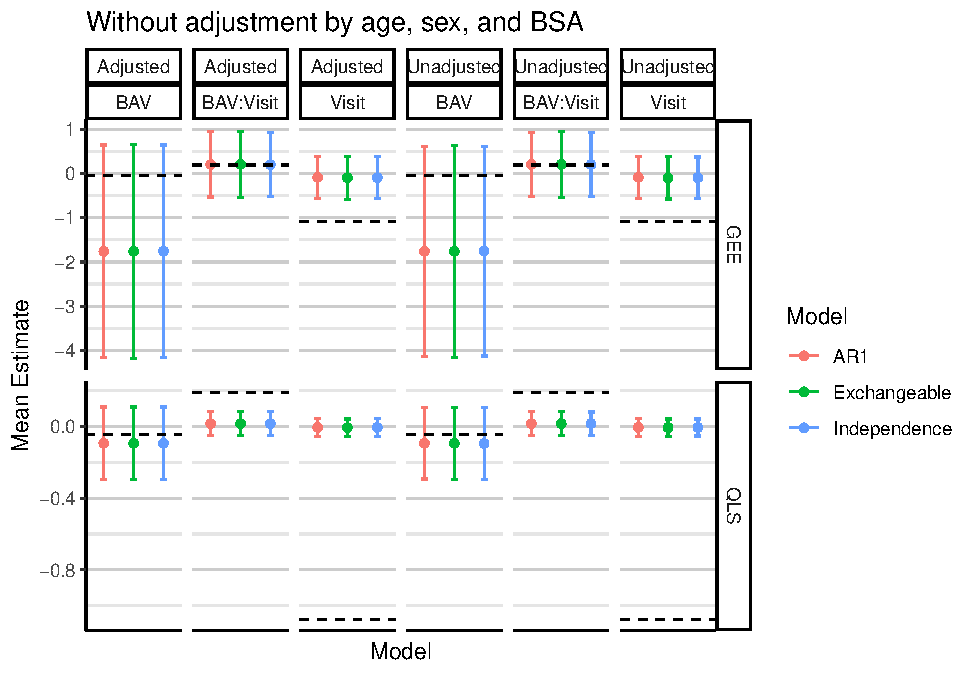
\includegraphics{FinalReport_files/figure-pdf/unnamed-chunk-4-1.pdf}

}

\caption{Relative bias of estimations for the effect of BAV using GEE
and QLS with independence, AR1, and exchangeable working correlation
structures.}

\end{figure}%

Figure 3 shows the plot of the relative bias of estimates for the
interaction effect between BAV and time. With the same layout as Figure
2, the GEE method still exhibits moderate variability with median values
around zero. In contrast, the QLS method shows low variability but
exhibits a negative relative bias, with estimates skewed below zero,
irrespective of including confounding covariates.

\begin{figure}[H]

{\centering 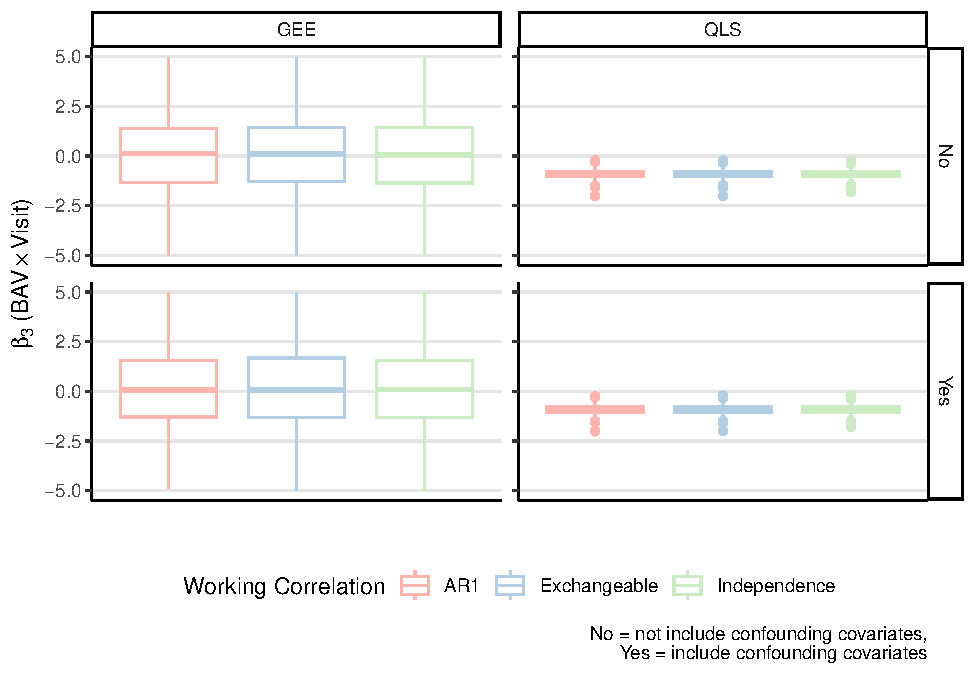
\includegraphics{FinalReport_files/figure-pdf/unnamed-chunk-5-1.pdf}

}

\caption{Relative bias of estimations for the interaction effect of BAV
and time using GEE and QLS with independence, AR1, and exchangeable
working correlation structures.}

\end{figure}%

The comparison of the mean estimation for correlations \(\alpha\) among
longitudinal measurements between GEE and QLS methods is shown in Table
2. Given that the true intravisit correlation is set to be 0.3, the GEE
method shows lower bias in the estimates of \(\alpha\), with a mean
value of 0.166, and it shows the closest value when the specification
working correlation is consistent with the true working correlation
structure. However, when the working correlation is specified to be
exchangeable, the GEE approach tends to underestimate the intravisit
correlation at around 0.1. In contrast, the QLS method provides more
consistent estimates across different covariate sets and working
correlations, at around 0.7, though with generally higher bias.

\begin{table}[H]
\centering\centering
\caption{\footnotesize Comparison of mean estimation for the correlation among longitudinal measurements using GEE and QLS methods, with and without adjustment for age, sex, and BSA.}
\centering
\resizebox{\ifdim\width>\linewidth\linewidth\else\width\fi}{!}{
\fontsize{8}{10}\selectfont
\begin{tabular}[t]{>{}llrrrrr}
\toprule
\multicolumn{2}{c}{ } & \multicolumn{2}{c}{GEE} & \multicolumn{1}{c}{ } & \multicolumn{2}{c}{QLS} \\
\cmidrule(l{3pt}r{3pt}){3-4} \cmidrule(l{3pt}r{3pt}){6-7}
Working Correlation & Covariate Set & Mean Estimate & Bias & True Value & Mean Estimate & Bias\\
\midrule
 & No & 0.246 & -0.054 & 0.3 & 0.727 & 0.427\\
\cmidrule{2-7}
\multirow[t]{-2}{*}[1\dimexpr\aboverulesep+\belowrulesep+\cmidrulewidth]{\raggedright\arraybackslash \textbf{AR1}} & Yes & 0.196 & -0.104 & 0.3 & 0.725 & 0.425\\
\cmidrule{1-7}
 & No & 0.130 & -0.170 & 0.3 & 0.561 & 0.261\\
\cmidrule{2-7}
\multirow[t]{-2}{*}[1\dimexpr\aboverulesep+\belowrulesep+\cmidrulewidth]{\raggedright\arraybackslash \textbf{Exchangeable}} & Yes & 0.095 & -0.205 & 0.3 & 0.725 & 0.425\\
\bottomrule
\multicolumn{7}{l}{\rule{0pt}{1em}\textsuperscript{*} Covariate Set: Yes = Included confounding covariates, No = Without confounding covariates}\\
\end{tabular}}
\end{table}

Table 3 presents the estimation of correlations (\(\tau\)) between
subjects in matched pairs using the QLS approach, across the three
different working correlations and covariate sets (with and without
confounder adjustment). In general, including confounding covariates
consistently have higher estimation irrespective of the specified
working correlation, although the difference is ignorable. When the
working correlation is specified correctly (AR1) and without including
confounding covariates, the estimation are the lowest at 0.361 with a
standard deviation of 0.137. With exchangeable working correlation, the
mean estimation is around 0.390 with a SD of 0.111. Finally, the mean
\(\tau\) is estimated to be 0.486 with a SD of 0.095 when the working
correlation is specified to be independence. Figure 4 visualized the
estimation for \(\tau\).

\begin{table}[H]
\centering\centering
\caption{\footnotesize Estimation of correlations between subjects in matched pairs using QLS approach.}
\centering
\resizebox{\ifdim\width>\linewidth\linewidth\else\width\fi}{!}{
\fontsize{8}{10}\selectfont
\begin{tabular}[t]{>{}llrr}
\toprule
Working Correlation & Covariate Set & Mean $\tau$ & SD $\tau$\\
\midrule
 & No & 0.361 & 0.137\\
\cmidrule{2-4}
\multirow[t]{-2}{*}{\raggedright\arraybackslash \textbf{AR1}} & Yes & 0.362 & 0.137\\
\cmidrule{1-4}
 & No & 0.389 & 0.111\\
\cmidrule{2-4}
\multirow[t]{-2}{*}{\raggedright\arraybackslash \textbf{Exchangeable}} & Yes & 0.390 & 0.111\\
\cmidrule{1-4}
 & No & 0.485 & 0.095\\
\cmidrule{2-4}
\multirow[t]{-2}{*}{\raggedright\arraybackslash \textbf{Independence}} & Yes & 0.487 & 0.094\\
\bottomrule
\multicolumn{4}{l}{\rule{0pt}{1em}\textsuperscript{*} Covariate Set: Yes = Included confounding covariates, No = Without confounding covariates}\\
\end{tabular}}
\end{table}

\begin{figure}[H]

{\centering 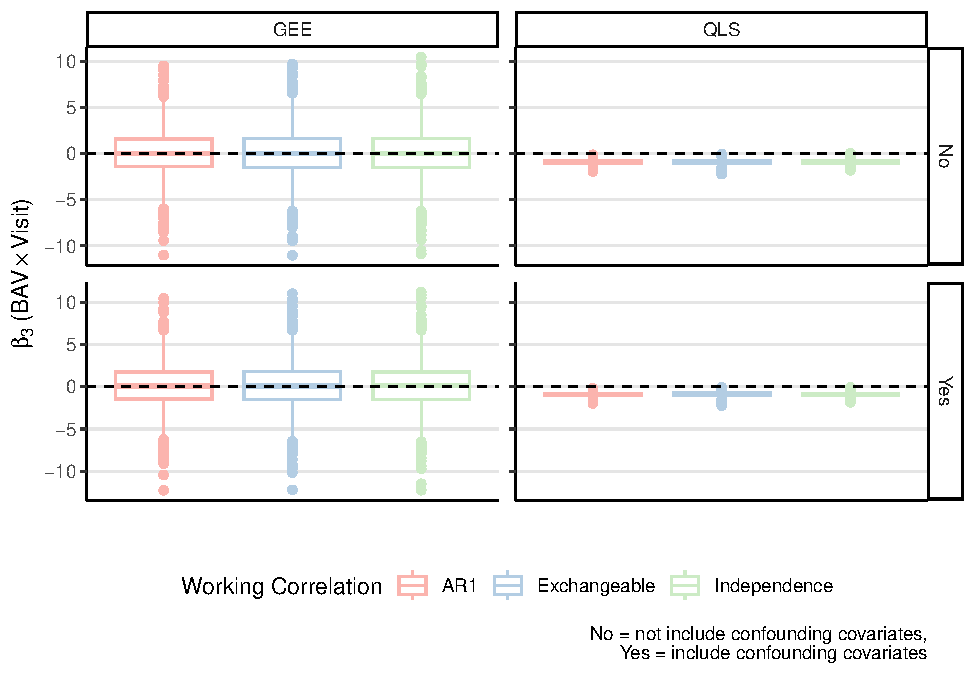
\includegraphics[width=0.7\textwidth,height=\textheight]{FinalReport_files/figure-pdf/unnamed-chunk-8-1.pdf}

}

\caption{Estimation of intra-pair correlation using QLS approach across
three different working correlation structures for both with and without
inclusion of confounding covariates.}

\end{figure}%

\section{Discusssion}\label{discusssion}

In this paper, we assessed the performance and validity of the
Generalized Estimating Equations (GEE) method and the two-stage
quasi-least squares (QLS) approach in analyzing small matched-pair
longitudinal binary data, particularly focusing on the effect of
bicuspid aortic valve (BAV) on aortic root size post-surgery. We
analyzed a cohort of patients from the Peter Munk Cardiac Center and
performed extensive simulations to compare these methods under different
working correlation structures. Our findings revealed no significant
difference in performance across different specified working
correlations, nor between the estimation results from the empirical
sandwich estimator and the corrected ones.

In our simulation study, the QLS method demonstrates superior
performance, with mean estimates closer to the true coefficients and
narrower confidence intervals than GEE. Moreover, GEE tends to
underestimate the intravisit correlation parameter (\(\alpha\)) with low
bias only when the working correlation is specified correctly. In
contrast, QLS provided more consistent estimates of \(\alpha\) across
different working correlation specifications, although biases are much
higher than those based on the GEE approach. Both methods failed to
capture the effect of time. Additionally, including confounding
covariates did not present large differences in performance. The
findings highlight the importance of choosing an appropriate correlation
structure in GEE analyses. For studies with small sample sizes and
complex correlation structures, QLS may offer a more reliable
alternative by providing consistent estimates with lower variability.

This study has several limitations. The small sample size of our
motivational data and the assumption of AR1 as the true correlation
structure may limit the generalizability of our findings. However, these
limitations also present exciting opportunities for future research to
explore alternative correlation structures and extend the QLS method to
accommodate more complex data scenarios. The informative dropout process
modeled in our simulations may not fully capture real-world
complexities, but it also motivates further investigations to refine GEE
and QLS approaches for handling informative dropouts and covariate
endogeneity in longitudinal studies.

In conclusion, our comparative analysis of GEE and QLS methods provides
valuable insights into their performance in analyzing longitudinal
binary data. While GEE showed better ability to capture the correlation
among repeated measurements, QLS demonstrated lower variability and
consistent parameter estimates across different correlation structures.
These robust findings underscore the importance of methodological
considerations in longitudinal data analysis and offer confident
guidance for researchers in selecting appropriate analytical approaches
for their studies.

\newpage

\section{Appendix A}\label{appendix-a}

\subsection{\texorpdfstring{Estimation for Stage One
\(\alpha\)}{Estimation for Stage One \textbackslash alpha}}\label{estimation-for-stage-one-alpha}

Since the maximum number repeated measurement within the same subject is
restricted to 6, we take \(t_{ij} = 4\) as an example for simplicity.
The intravisit correlation structure is \[
R_i(\alpha) = 
\begin{bmatrix}
1 & \alpha & \alpha^2 & \alpha^3\\
\alpha & 1 & \alpha & \alpha^2\\
\alpha^2 & \alpha & 1 & \alpha\\
\alpha^3 & \alpha^2 & \alpha & 1
\end{bmatrix}
\] The partial derivative of covariance matrix with respect to
\(\alpha\) is \[
\frac{\partial F_i^{-1}(\alpha)}{\partial \alpha} = \frac{\partial{R_i^{-1}(\alpha)}}{\partial \alpha} \otimes Q_i^{-1}(\tau)
\] because \(Q^{-1}_i(\tau)\) does not contain \(\alpha\). \[
\frac{\partial{R_i^{-1}(\alpha)}}{\partial \alpha} = -R_i^{-1}(\alpha) \frac{\partial R_i(\alpha)}{\partial \alpha} R_i^{-1}(\alpha)
\]

\[
\frac{\partial R_i(\alpha)}{\partial \alpha}= 
\begin{bmatrix}
0 & 1 & 2\alpha & 3\alpha^2\\
1 & 0 & 1 & 2\alpha\\
2\alpha & 1 & 0 & 1\\
3\alpha^2 & 2\alpha & 1 & 0
\end{bmatrix}
\] Therefore, \[
\frac{\partial{R_i^{-1}(\alpha)}}{\partial \alpha}= 
\frac{1}{(1-\alpha^2)^2}
\begin{bmatrix}
2\alpha & -(1+\alpha^2) & 0 & 0\\
-(1+\alpha^2) & 4\alpha & -(1+\alpha^2) & 0\\
0 & -(1+\alpha^2) & 4\alpha & -(1+\alpha^2)\\
0 & 0 & -(1+\alpha^2) & 0
\end{bmatrix}
\] \[
\frac{\partial{R_i^{-1}(\alpha)}}{\partial \alpha}\otimes Q_i^{-1} = 
\frac{1}{(1-\alpha^2)^2}
\begin{bmatrix}
2\alpha Q_i^{-1} & -(1+\alpha^2) Q_i^{-1} & 0 & 0\\
-(1+\alpha^2) Q_i^{-1} & 4\alpha Q_i^{-1} & -(1+\alpha^2) Q_i^{-1} & 0\\
0 & -(1+\alpha^2) Q_i^{-1} & 4\alpha Q_i^{-1} & -(1+\alpha^2) Q_i^{-1}\\
0 & 0 & -(1+\alpha^2) Q_i^{-1} & 2\alpha Q_i^{-1}
\end{bmatrix}
\] Hence, \[
\begin{aligned}
\frac{\partial Q(\beta, \Gamma)}{\partial \alpha} &= 
\sum_{i=1}^m \sum_{j=1}^2 
\begin{pmatrix}
Z_{i1} & Z_{i2} & Z_{i3} & Z_{i4} 
\end{pmatrix}
\frac{\partial{R_i^{-1}(\alpha)}}{\partial \alpha}\otimes Q_i^{-1}
\begin{pmatrix}
Z_{i1} \\ Z_{i2} \\ Z_{i3} \\ Z_{i4} 
\end{pmatrix}\\
&= \frac{1}{(1-\alpha^2)^2} \sum_{i=1}^m \sum_{j=1}^2 
\Big\{2\alpha \Big(Z_{ij1}Q_i^{-1}Z_{ij1} + 2Z_{ij2}Q_i^{-1}Z_{ij2}+  2Z_{ij3}Q_i^{-1}Z_{ij3}+Z_{ij4}Q_i^{-1}Z_{ij4}\Big)\\
& \quad \quad \quad \quad \quad\quad 2(1+\alpha^2)\cdot 
\Big(Z_{ij1}Q_i^{-1}Z_{ij2}+Z_{ij2}Q_i^{-1}Z_{ij3}+Z_{ij3}Q_i^{-1}Z_{ij4}\Big)
\Big\}\\
&= \sum_{i=1}^m \sum_{j=1}^2 \left\{\alpha 
\left(\sum_{k=1}^{t_{ij}} Z_{ijk}'Q_i^{-1} Z_{ijk} + \sum_{k=2}^{t_{ij} - 1}Z_{ijk}'Q_i^{-1} Z_{ijk}\right) - (1+\alpha^2)\left(\sum_{k=1}^{t_{ij} - 1}Z_{ijk}'Q_i^{-1}Z_{ijk+1}\right) \right\}
\end{aligned}
\] Let
\(S_1 = \sum_{k=1}^{t_{ij}} Z_{ijk}'Q_i^{-1} Z_{ijk} + \sum_{k=2}^{t_{ij} - 1}Z_{ijk}'Q_i^{-1} Z_{ijk}\)
and \(S_2 = \sum_{k=1}^{t_{ij} - 1}Z_{ijk}'Q_i^{-1}Z_{ijk+1}\), then \[
\begin{aligned}
\frac{\partial Q(\beta, \Gamma)}{\partial \alpha} &= \sum_{i=1}^m \sum_{j=1}^2 \big(\alpha S_1 - (1+\alpha^2) S_2\big) \\
&= \sum_{i=1}^m \sum_{j=1}^2\big(\alpha S_1 - S_2-\alpha^2S_2\big) = 0\\
& \sum_{i=1}^m \sum_{j=1}^2\big(\alpha^2 S_2 -\alpha S_1 + S_2\big) = 0\\
\hat{\alpha}_0 &= \sum_{i=1}^m \sum_{j=1}^2\frac{S_1+\sqrt{S_1^2+4S_2^2}}{2S_2}
\end{aligned}
\]

\newpage

\section{Appendix B}\label{appendix-b}

\subsection{Coverage Probability}\label{coverage-probability}

\begin{table}[!h]
\centering\centering
\caption{\footnotesize The Coverage Probability of Regression Coefficient Estimation from GEE and QLS.}
\centering
\resizebox{\ifdim\width>\linewidth\linewidth\else\width\fi}{!}{
\fontsize{8}{10}\selectfont
\begin{tabular}[t]{lrrrrrrrr}
\toprule
\multicolumn{1}{c}{ } & \multicolumn{4}{c}{GEE} & \multicolumn{4}{c}{QLS} \\
\cmidrule(l{3pt}r{3pt}){2-5} \cmidrule(l{3pt}r{3pt}){6-9}
Term & Empirical SE & DF-SE & Empirical SE & DF-SE & Empirical SE & DF-SE & Empirical SE & DF-SE\\
\midrule
(Intercept) & 0.879 & 0.888 & 0.909 & 0.913 & 1.000 & 1.000 & 0.001 & 0.001\\
bav & 0.816 & 0.829 & 0.821 & 0.828 & 1.000 & 1.000 & 1.000 & 1.000\\
bav:visit & 0.861 & 0.865 & 0.861 & 0.863 & 1.000 & 1.000 & 1.000 & 1.000\\
visit & 0.107 & 0.108 & 0.087 & 0.088 & 0.000 & 0.000 & 0.000 & 0.000\\
(Intercept) & 0.876 & 0.892 & 0.918 & 0.920 & 0.974 & 0.976 & 0.000 & 0.000\\
\addlinespace
bav & 0.820 & 0.832 & 0.830 & 0.835 & 1.000 & 1.000 & 1.000 & 1.000\\
bav:visit & 0.870 & 0.878 & 0.889 & 0.891 & 0.984 & 0.984 & 0.980 & 0.981\\
visit & 0.108 & 0.111 & 0.087 & 0.088 & 0.000 & 0.000 & 0.000 & 0.000\\
(Intercept) & 0.879 & 0.890 & 0.907 & 0.910 & 0.935 & 0.939 & 0.001 & 0.001\\
bav & 0.811 & 0.823 & 0.821 & 0.823 & 1.000 & 1.000 & 1.000 & 1.000\\
\addlinespace
bav:visit & 0.860 & 0.864 & 0.869 & 0.871 & 0.916 & 0.920 & 0.910 & 0.913\\
visit & 0.112 & 0.122 & 0.100 & 0.104 & 0.000 & 0.000 & 0.000 & 0.000\\
\bottomrule
\end{tabular}}
\end{table}

\subsection{Simulation Results}\label{simulation-results-1}

\begin{table}[!h]
\centering\centering\begingroup\fontsize{8}{10}\selectfont

\resizebox{\ifdim\width>\linewidth\linewidth\else\width\fi}{!}{
\begin{tabular}{>{}llllrrrrrr}
\toprule
  & Corstr & Type & Term & True Value & Mean Est & SD Est & Mean SE & Mean SE-DF & Mean MSE\\
\midrule
\textbf{1} &  & GEE & Intercept & -1.784 & -2.116 & 4.173 & 2.827 & 2.887 & 17.528\\
\cmidrule{1-1}
\cmidrule{3-10}
\textbf{3} &  & GEE & BAV & -0.042 & -1.595 & 7.357 & 1.255 & 1.281 & 56.538\\
\cmidrule{1-1}
\cmidrule{3-10}
\textbf{4} &  & GEE & BAV:Visit & 0.192 & 0.149 & 2.163 & 0.390 & 0.398 & 4.682\\
\cmidrule{1-1}
\cmidrule{3-10}
\textbf{7} &  & GEE & Visit & -1.077 & -0.019 & 2.138 & 0.256 & 0.261 & 5.691\\
\cmidrule{1-1}
\cmidrule{3-10}
\textbf{8} &  & QLS & Intercept & -1.784 & 0.128 & 0.315 & 2.012 & 2.055 & 3.755\\
\cmidrule{1-1}
\cmidrule{3-10}
\textbf{10} &  & QLS & BAV & -0.042 & -0.093 & 0.117 & 0.509 & 0.520 & 0.016\\
\cmidrule{1-1}
\cmidrule{3-10}
\textbf{11} &  & QLS & BAV:Visit & 0.192 & 0.017 & 0.042 & 0.192 & 0.196 & 0.032\\
\cmidrule{1-1}
\cmidrule{3-10}
\textbf{14} & \multirow[t]{-8}{*}{\raggedright\arraybackslash AR1} & QLS & Visit & -1.077 & -0.005 & 0.031 & 0.138 & 0.141 & 1.151\\
\bottomrule
\multicolumn{10}{l}{\rule{0pt}{1em}\textit{Corstr: } \textsuperscript{*} Correlation Structure}\\
\end{tabular}}
\endgroup{}
\end{table}

\begin{table}[!h]
\centering\centering\begingroup\fontsize{8}{10}\selectfont

\resizebox{\ifdim\width>\linewidth\linewidth\else\width\fi}{!}{
\begin{tabular}{>{}llllrrrrrr}
\toprule
  & Corstr & Type & Term & True Value & Mean Est & SD Est & Mean SE & Mean SE-DF & Mean MSE\\
\midrule
\textbf{1} &  & GEE & Intercept & -1.784 & -2.113 & 4.219 & 2.843 & 2.903 & 17.907\\
\cmidrule{1-1}
\cmidrule{3-10}
\textbf{3} &  & GEE & BAV & -0.042 & -1.586 & 7.526 & 1.262 & 1.288 & 59.021\\
\cmidrule{1-1}
\cmidrule{3-10}
\textbf{4} &  & GEE & BAV:Visit & 0.192 & 0.147 & 2.268 & 0.394 & 0.403 & 5.148\\
\cmidrule{1-1}
\cmidrule{3-10}
\textbf{7} &  & GEE & Visit & -1.077 & -0.027 & 2.177 & 0.258 & 0.263 & 5.840\\
\cmidrule{1-1}
\cmidrule{3-10}
\textbf{8} &  & QLS & Intercept & -1.784 & 0.127 & 0.314 & 1.701 & 1.738 & 3.749\\
\cmidrule{1-1}
\cmidrule{3-10}
\textbf{10} &  & QLS & BAV & -0.042 & -0.094 & 0.116 & 0.438 & 0.447 & 0.016\\
\cmidrule{1-1}
\cmidrule{3-10}
\textbf{11} &  & QLS & BAV:Visit & 0.192 & 0.018 & 0.042 & 0.155 & 0.159 & 0.032\\
\cmidrule{1-1}
\cmidrule{3-10}
\textbf{14} & \multirow[t]{-8}{*}{\raggedright\arraybackslash Exchangeable} & QLS & Visit & -1.077 & -0.007 & 0.032 & 0.111 & 0.114 & 1.146\\
\bottomrule
\multicolumn{10}{l}{\rule{0pt}{1em}\textit{Corstr:} \textsuperscript{*} Correlation Structure}\\
\end{tabular}}
\endgroup{}
\end{table}

\begin{table}[!h]
\centering\centering\begingroup\fontsize{8}{10}\selectfont

\resizebox{\ifdim\width>\linewidth\linewidth\else\width\fi}{!}{
\begin{tabular}{>{}llllrrrrrr}
\toprule
  & Corstr & Type & Term & True Value & Mean Est & SD Est & Mean SE & Mean SE-DF & Mean MSE\\
\midrule
\textbf{1} &  & GEE & Intercept & -1.784 & -2.062 & 4.207 & 2.823 & 2.883 & 17.778\\
\cmidrule{1-1}
\cmidrule{3-10}
\textbf{3} &  & GEE & BAV & -0.042 & -1.583 & 7.450 & 1.255 & 1.281 & 57.873\\
\cmidrule{1-1}
\cmidrule{3-10}
\textbf{4} &  & GEE & BAV:Visit & 0.192 & 0.145 & 2.209 & 0.385 & 0.393 & 4.882\\
\cmidrule{1-1}
\cmidrule{3-10}
\textbf{7} &  & GEE & Visit & -1.077 & -0.023 & 2.174 & 0.253 & 0.259 & 5.837\\
\cmidrule{1-1}
\cmidrule{3-10}
\textbf{8} &  & QLS & Intercept & -1.784 & 0.131 & 0.318 & 2.753 & 2.812 & 3.769\\
\cmidrule{1-1}
\cmidrule{3-10}
\textbf{10} &  & QLS & BAV & -0.042 & -0.094 & 0.114 & 0.524 & 0.535 & 0.016\\
\cmidrule{1-1}
\cmidrule{3-10}
\textbf{11} &  & QLS & BAV:Visit & 0.192 & 0.017 & 0.039 & 0.246 & 0.251 & 0.032\\
\cmidrule{1-1}
\cmidrule{3-10}
\textbf{14} & \multirow[t]{-8}{*}{\raggedright\arraybackslash Independence} & QLS & Visit & -1.077 & -0.005 & 0.029 & 0.172 & 0.175 & 1.150\\
\bottomrule
\multicolumn{10}{l}{\rule{0pt}{1em}\textit{Corstr, SD, MSE: } \textsuperscript{*} Correlation Structure, Standard Deviation and Mean Squared Error}\\
\end{tabular}}
\endgroup{}
\end{table}

\newpage


  \bibliography{bibliography.bib}



\end{document}
